\documentclass[10pt,a4paper,titlepage]{report}
\usepackage[utf8]{inputenc}
\usepackage{amsmath}
\usepackage{amsfonts}
\usepackage{amssymb}
\usepackage{graphicx}
\usepackage{xcolor}
\usepackage{minted}
\nonstopmode


\begin{document}
\begin{titlepage}
\author{Rwithik Manoj}
\title{Shell Scripting\\Set 2}
\date{\today}
\maketitle
\end{titlepage}

\begin{enumerate}
\item Write a shell script that displays a special listing showing the permissions, size filename and last modification time of filename supplied as arguments. Provide suitable headers using the printf command. \newline
\textbf{Algorithm}:\newline
\begin{enumerate}
	\item Start.
	\item Check if the file exists.
	\item If it does, print its details with {\color{red}ls -l}.
	\item Stop.
\end{enumerate}
\newline
\textbf{Script:}\newline
\inputminted{bash}{../Scripts/Set2/1.sh}
\newline
\textbf{Output:}\newline
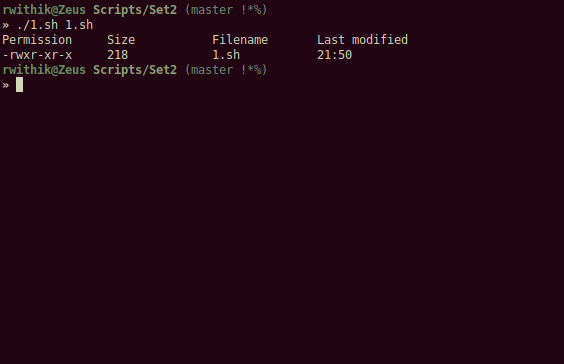
\includegraphics[width=\linewidth]{../Images/Shell2/1.png}
\pagebreak

\item Write a script that compares two directories dir1 and dir2(supplied as arguments) and copies to dir1 from dir2 every file that is not present in dir1. \newline
\textbf{Algorithm}:\newline
\begin{enumerate}
	\item Start.
	\item Check if both the directories exist.
	\item If it does, copy the contents using {\color{red}cp -n} flag.
	\item Stop.
\end{enumerate}
\newline
\textbf{Script:}\newline
\inputminted{bash}{../Scripts/Set2/2.sh}
\newline
\textbf{Output:}\newline
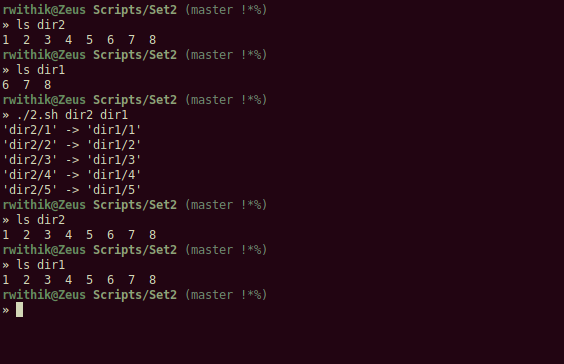
\includegraphics[width=\linewidth]{../Images/Shell2/2.png}
\pagebreak

\item Write a shell script that accepts two file names as arguments, checks if the permissions for these files are identical and if the permissions are identical,output common permissions and otherwise output each file name followed by its permissions. \newline
\textbf{Algorithm}:\newline
\begin{enumerate}
	\item Start.
	\item Exit the script if the files don't exist.
	\item Get the permissions of the files with {\color{red}awk} and {\color{red}ls -l}.
	\item If the permissions are same, print that they are equal, else print the permissions.
	\item Stop.
\end{enumerate}
\newline
\textbf{Script:}\newline
\inputminted{bash}{../Scripts/Set2/3.sh}
\newline
\textbf{Output:}\newline
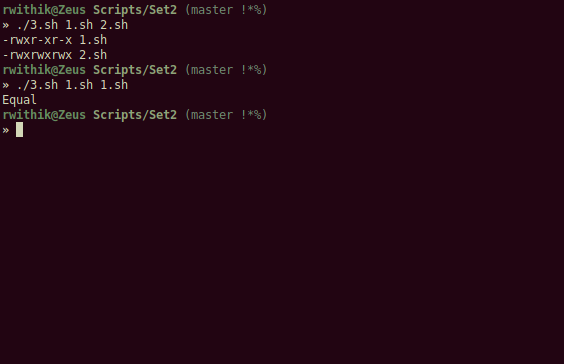
\includegraphics[width=\linewidth]{../Images/Shell2/3.png}
\pagebreak

\item Write a shell script which receives two file names as arguments. It should check whether the two file contents are same or not. If they are same then second file should be deleted. \newline
\textbf{Algorithm}:\newline
\begin{enumerate}
	\item Start.
	\item Exit the script if the files don't exist.
	\item Check if the files are the same with {\color{red}diff}.
	\item If the contents are the same, delete the second file.
	\item Stop.
\end{enumerate}
\newline
\textbf{Script:}\newline
\inputminted{bash}{../Scripts/Set2/4.sh}
\newline
\textbf{Output:}\newline
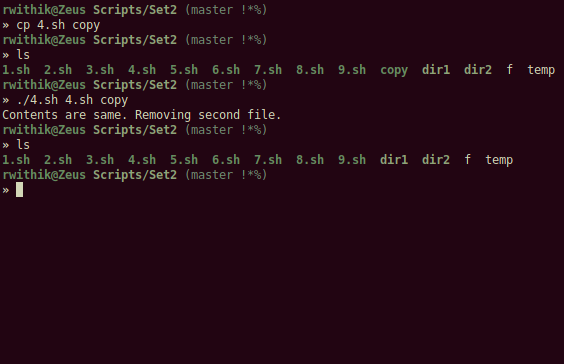
\includegraphics[width=\linewidth]{../Images/Shell2/4.png}
\pagebreak

\item Write a shell script that, given a file name as the argument will count vowels, blank spaces, characters, number of line and symbols. \newline
\textbf{Algorithm}:\newline
\begin{enumerate}
	\item Start.
	\item Exit the script if the file does not exist.
	\item Count the number of vowels using {\color{red}cat}, {\color{red}grep} and {\color{red}wc}.
	\item Count the number of characters using {\color{red}wc -c}.
	\item Count the number of blank lines by searching for the pattern ``\^{}\$''. \^{} matches the beginning of a line, and \$ matches the end of a line. So the pattern matches the lines in which the beginning and end are adjacent, ie blank lines.
	\item Count the number of lines using {\color{red}wc -l}.
	\item Stop.
\end{enumerate}
\newline
\textbf{Script:}\newline
\inputminted{bash}{../Scripts/Set2/5.sh}
\newline
\textbf{Output:}\newline
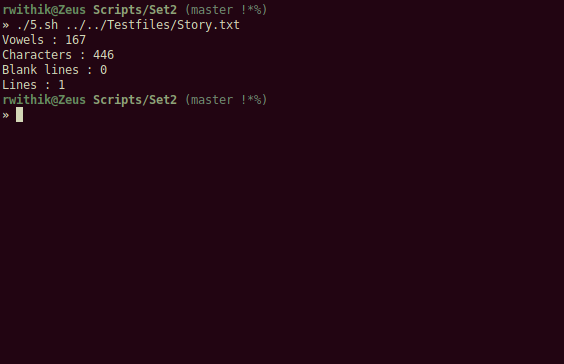
\includegraphics[width=\linewidth]{../Images/Shell2/5.png}
\pagebreak
\item Write a shell script that will take an input file and remove identical lines. \newline
\textbf{Algorithm}:\newline
\begin{enumerate}
	\item Start.
	\item Exit the script if the file does not exist.
	\item Use {\color{red}awk `!seen[\$0]++' }.
	\item This makes a dictionary, named seen. When a new line is encountered, it sets the value of the key as one. It prints the lie only if the value of seen[\$0] is zero. So the next time the same line is encountered, it is not printed.
	\item Stop.
\end{enumerate}
\newline
\textbf{Script:}\newline
\inputminted{bash}{../Scripts/Set2/6.sh}
\pagebreak
\item Write a shell script that displays a list of all the files in the current directory to which the user has read, write and execute permissions. \newline
\textbf{Algorithm}:\newline
\begin{enumerate}
	\item Start.
	\item Write the contents of the current directory to a file, f.
	\item Redirect the input stream to the file.
	\item Check the permissions of the file with the {\color{red}-r}, {\color{red}-w}and {\color{red}-x} flags of {\color{red}test}.
	\item Stop.
\end{enumerate}
\newline
\textbf{Script:}\newline
\inputminted{bash}{../Scripts/Set2/7.sh}
\newline
\textbf{Output:}\newline
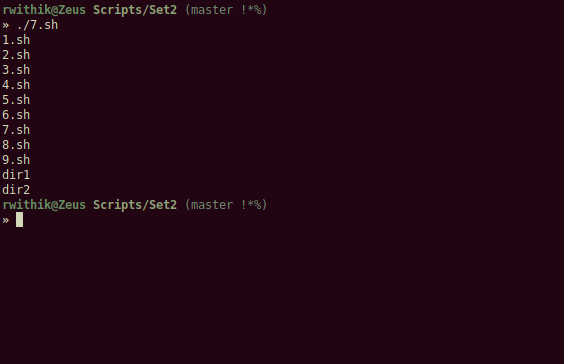
\includegraphics[width=\linewidth]{../Images/Shell2/7.png}
\pagebreak

\item Write a shell script that folds long lines into 40 columns. Thus any line that exceeds 40 characters must be broken after 40th. A \textbackslash  is to be appended as the indication of folding and the processing is to be continued with the residue. The input is to be through a text file created by the user. \newline
\textbf{Algorithm}:\newline
\begin{enumerate}
	\item Start.
	\item Exit the script if the file doesn't exist.
	\item Store the number of characters in a variable, n.
	\item Loop through the file and cut 40 characters in each iteration.
	\item Stop.
\end{enumerate}
\newline
\textbf{Script:}\newline
\inputminted{bash}{../Scripts/Set2/8.sh}
\newline
\textbf{Output:}\newline
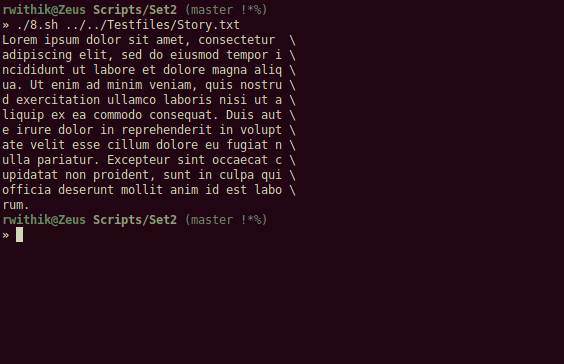
\includegraphics[width=\linewidth]{../Images/Shell2/8.png}
\pagebreak

\item Write a shell script to delete all lines containing a specific word in one or more file supplied as argument to it. \newline
\textbf{Algorithm}:\newline
\begin{enumerate}
	\item Start.
	\item Read the word.
	\item Loop through the files.
	\item Check of the file exists.
	\item Delete the lines contaning the word, with {\color{red}sed}.
	\item Stop.
\end{enumerate}
\newline
\textbf{Script:}\newline
\inputminted{bash}{../Scripts/Set2/9.sh}
\newline
\textbf{Output:}\newline
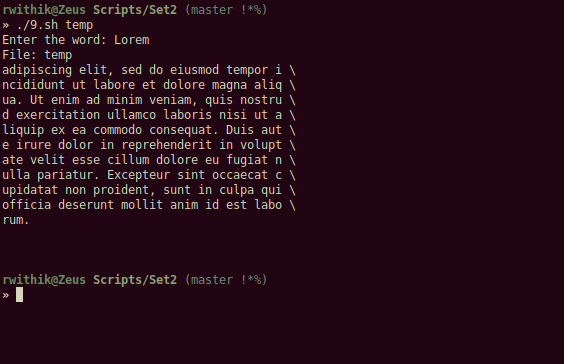
\includegraphics[width=\linewidth]{../Images/Shell2/9.png}
\end{enumerate}

\end{document} 
